\section{Implementation}
\label{sec:implementation}

The Django\cite{django} Web application development framework and the Web API toolkit for Django, Django REST Framework\cite{drf}, were used to develop our annotation tool.
PostgreSQL\cite{psql} is used to provide a database for the server-side applications of the software.
This database is responsible for serving the entire data needed to operate the tool, the search API, etc.
During the implementation phase, decisions regarding models in the database have been directed towards making the tool use the API for database queries and searches.
The models reflect the UD format of a sentence and sentences are saved as word lines at the core.

Annotation page has all the functionalities of BoAT v1 and more.
Errors are included for annotators to see invalid edits in real time.
They are checked and annotations validated according to the UD framework and the language provided.
The scripts used for validation are the latest ones already provided by the framework.\cite{UD-git}

A Python library \textit{spaCy}\cite{spacy} is used to provide linear dependency graphs.
Another JavaScript-based linear dependency graph\cite{spyssalo} making use of brat\cite{brat-vis} is used to provide graphs as well.
The preferences of annotators may vary and giving them options in different parts of the screen is important.

\begin{figure}[tbh]
    \centering
    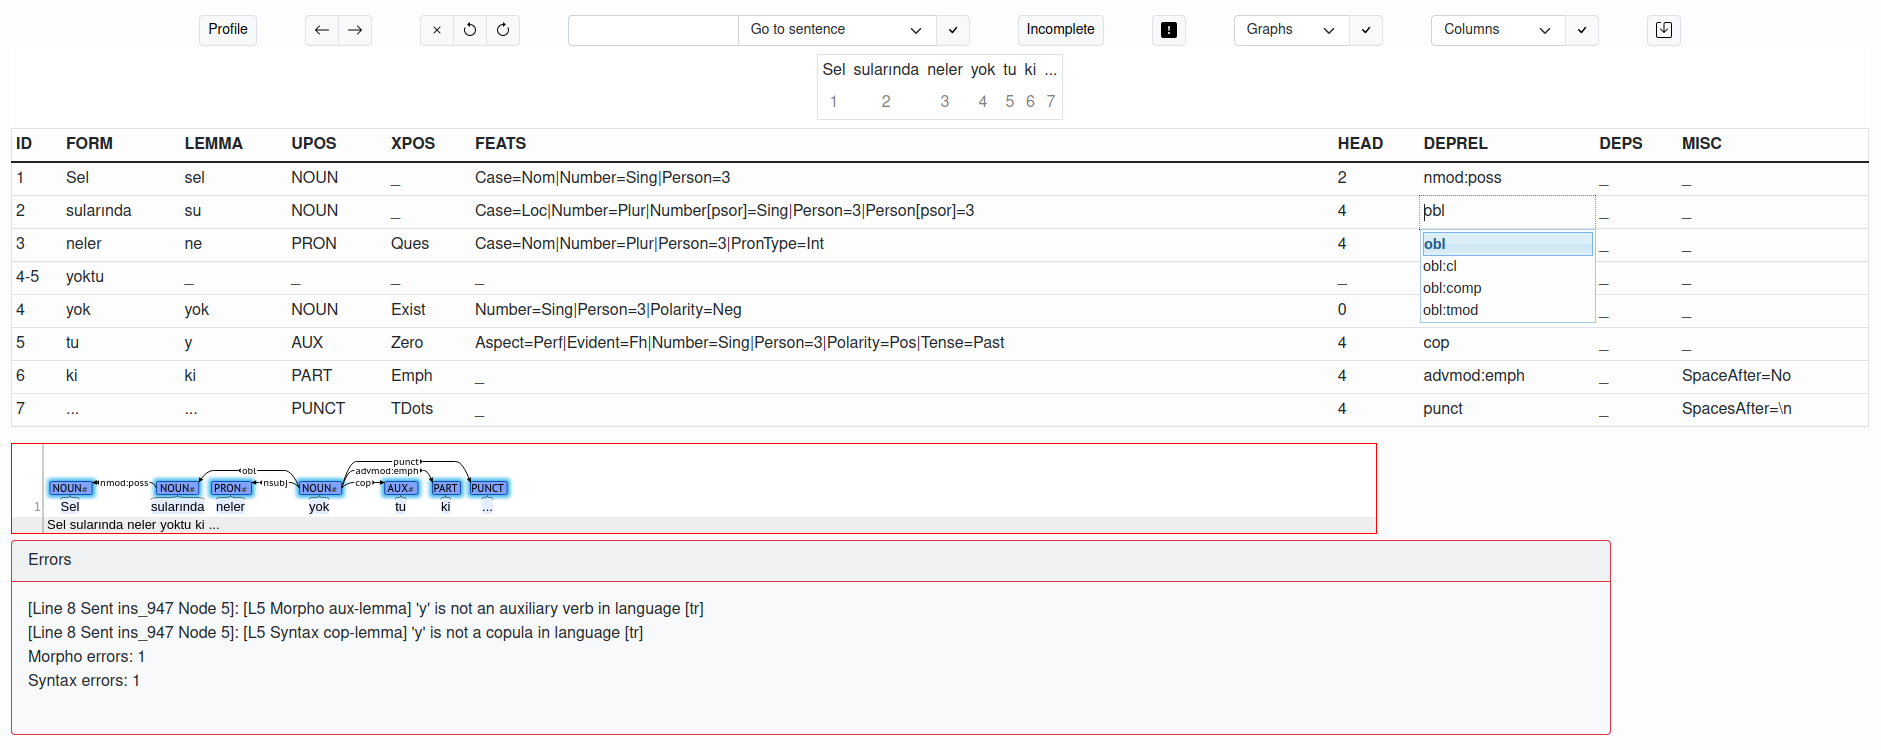
\includegraphics[width=1\textwidth]{figures/1.png}
    \caption{Annotation view for a sentence being annotated.}
    \label{fig:demo-fig}
\end{figure}

\subsection{API}
\label{sec:api}

By using our annotated treebank search API, other parties wanting to see the capabilities of the tool can retrieve our annotated treebanks.
Also, some parties wanting to use the treebanks in their computation tasks can easily extract information from our treebanks by using the API.
This opens up many possibilities for the use of the tool beyond the annotator's UI experience.
We plan to dockerize the tool and make it accessible, following development practices and conventions.

\subsection{Demo}
\label{sec:demo}

A demo will be provided on our university's NLP web page where the annotation capabilities of the tool built can be tested.
